\documentclass[12pt]{article}

\usepackage[spanish]{babel}
\usepackage{hyperref}
\usepackage{graphicx}
\usepackage{listings}
\usepackage{color}
\usepackage{multicol}
\usepackage{amssymb}
\usepackage{enumitem}
\usepackage{here}
\usepackage{dsfont}
\usepackage{amsmath}
\usepackage{tipa}
\usepackage{float}
\spanishdecimal{.}

\title{Matemáticas para las Ciencias Aplicadas I}
\title{
	Cuarta Lista de Problemas \\
	\textbf{Primera  Parte} \\
	\vspace{1ex}
	\large Matemáticas para las Ciencias Aplicadas I \\
	Facultad de Ciencias, UNAM}

\date{\today}

\author{Flores Morán Julieta Melina \\ Zarco Romero José Antonio}

%% Sección 5.3: 44 y 73.
%% Sección 5.5: 28 y 37.
%% Sección 5.6: 58, 63 y 70.
%% Sección 5.8: 27.
%% Sección 5.9: 52 y 64

\begin{document}

\maketitle

%% 5.3 -----------------------------------------------------------------------------------------------------------------------------------------------------------------------------------------------------------------------------
\section{Sección 5.3 \\ Integración Por Sustitución}
% 44 -------------------------------------------------------------------------------------------------------------
\subsection{Ejercicio 44} Flores Morán Julieta Melina \\

Evaluar las integrales utilizando sustituciones apropiadas.
\[
\int \tan^3{5x}\sec^2{5x}dx
\]
Tomemos $u = \tan5x \rightarrow du = 5 \sec^{2}5xdx \rightarrow \frac{du}{5} = \sec^{2}5xdx $. \\
Sustituimos en la integral:
\[
\int u^3 \frac{du}{5}
\]
Y resolvemos normalmente:\\
\begin{align*}
  \int u^3 \frac{du}{5}
  & = \int u^3 du \frac{1}{5} \\
  & = \frac{1}{5} \int u^3 du \\
  & = \frac{1}{5} \frac {u^4}{4} + C \\
  & = \frac {u^4}{20} + C\\
\end{align*}
y regresamos a u a su valor original.
\begin{align*}
  \frac {u^4}{20} + C 
  & = \frac{\tan^45x}{20} + C
\end{align*}
% 73 -------------------------------------------------------------------------------------------------------------
\subsection{Ejercicio 73} name \\

\begin{enumerate}[label=(\alph*)]
\item Evalúe $\int \rigth[ \frac {x}{\sqrt{x^2+1}}  \left] dx$

\item Utilice una herramienta gráfica para generar algunas curvas integrales típicas de $f(x) = x / \sqrt{x^2 + 1|1}$ en el intervalo $(-5, 5)$.
  
\end{enumerate}

%% 5.5 -----------------------------------------------------------------------------------------------------------------------------------------------------------------------------------------------------------------------------
\section{Sección 5.5 \\ La Integral Definida}
% 28 -------------------------------------------------------------------------------------------------------------
\subsection{Ejercicio 28} Flores Morán Julieta Melina \\

Utilice el Teorema 5.5.4 y fórmulas apropiadas de geometría para evaluar las integrales. \\

\[
\int_{-3}^{0} \left(2+\sqrt{9-x^2} \right)dx
\]
Siguiendo el teorema 5.5.4, esta integral equivale a : \\
\[
\int_{-3}^{0}  2 dx +  \int_{-3}^{0} \sqrt{9-x^2} \right)dx
\]
Procedamos a evaluar la primera integral $\int_{-3}^{0} 2 dx$ donde podemos ver la función $y=2$ que es una línea recta horizontal, por lo que el área formada con el eje x en el intervalo de 0 a -3 es un rectángulo de altura 2 y de base $|-3| = 3$, así que el área es $3 \cdot 2$ y entonces
\[
\int_{-3}^{0}  2 dx  = 6
\]
Para la segunda integral  $ \int_{-3}^{0} \sqrt{9-x^2}\right)dx$. Tenemos que  $y = \sqrt{9-x^2}  $ delimita la región de un cuarto de un circulo donde $r^2 = 9$ y por lo tanto su radio es de 3. \\ Considerando la formular del área de un circulo tenemos que el área de la cuarta parte es $\frac{1}{4} \pi (3)^2$, por lo tanto.
\[
 \int_{-3}^{0} \sqrt{9-x^2} \right)dx  = \frac{9\pi}{4}
 \]
 Por lo tanto el resultado de la suma de ambas sería: \\
 \[
\int_{-3}^{0}  2 dx +  \int_{-3}^{0} \sqrt{9-x^2}\right)dx = 6 + \frac{9\pi}{4} 
\]
Lo que resuelve la integral dada.
\[
\int_{-3}^{0} \left(2+\sqrt{9-x^2}\right)dx  = 6 + \frac{9\pi}{4} 
\]
% 37 -------------------------------------------------------------------------------------------------------------
\subsection{Ejercicio 37} name \\

Evaluar las integrales completando el cuadrado y aplicando fórmulas apropiadas de geometría.
\[
\int_{0}^{10} \sqrt{10x-x^2}dx
\]

%% 5.6 -----------------------------------------------------------------------------------------------------------------------------------------------------------------------------------------------------------------------------
\section{Sección 5.6 \\ El Teorema Fundamental Del Cálculo}
% 58 -------------------------------------------------------------------------------------------------------------
\subsection{Ejercicio 58} Flores Morán Julieta Melina \\

Defina $F (x)$ por
\[
F(x)=\int_{\pi/4}^{x} \cos{2t} dt
\]
\begin{enumerate}[label=(\alph*)]
\item Utilice la parte 2 del teorema fundamental del cálculo para encontrar $F'(x)$. \\
  La parte 2 del teorema fundamental del cálculo nos dice que $\frac{d}{dx}\left[ \int_{a}^{x} f(t)dt \right] = f(x)$. En este caso el integrando es una función continua, entonces $f(x) = cos2x$. Por lo tanto $F'(x) = \cos{2x}$
\item Verifique el resultado del inciso (a) integrando primero y luego diferenciando. \\
Podemos resolver la integral mediante un cambio de variable. $u= 2t \rightarrow du = 2dt  \rightarrow dt = \frac{du}{2}$\\
\begin{align*}
  F(x)
  & = \int_{\pi/4}^{x} \cos{2t} dt \\
  & = \int_{u(\pi/4)}^{u(x)} \cos{u} \frac{du}{2}\\
  & = \frac{1}{2} \int_{\pi/2}^{2x} \cos{u} du \\
  & = \frac{1}{2} \sen u \Bigg|_{\pi/2}^{2x} \\
  & = \frac{1}{2} \left[  \sen 2x - \sen \frac{\pi}{2} \right] \\
  & = \frac{1}{2} \left[  \sen 2x - 1 \right]\\
  & = \frac{1}{2}  \sen 2x - \frac{1}{2}  
\end{align*}
Y ahora podemos derivar $F(x)$.
\begin{align*}
  F'(x)=
  & = \frac{d}{dx} \left[ \frac{1}{2}  \sen 2x - \frac{1}{2} \right]  \\
  & = \frac{1}{2}  \cos 2x \cdot 2 \\
  & = \cos 2x  \\
\end{align*}
\end{enumerate}

% 63 -------------------------------------------------------------------------------------------------------------
\subsection{Ejercicio 63} name \\

Sea $F(x)=\int_{4}^{x} \sqrt{t^2+9}dt$. Encuentre
\begin{enumerate}[label=(\alph*)]
\item $F(4)$.
  
\item $F'(4)$.
  
\item $F''(4)$.
  
\end{enumerate}

% 70 -------------------------------------------------------------------------------------------------------------
\subsection{Ejercicio 70} Flores Morán Julieta Melina \\

Un ingeniero de tránsito monitorea la velocidad a la que los automóviles ingresan a la carretera principal durante la hora pico de la tarde. De sus datos estima que entre las 16:30 horas. y 17:30 p.m. la tasa  $R(t)$ a la que los automóviles ingresan a la carretera está dada por la fórmula $R(t) = 100 (1$ - $0.0001t^2 )$ automóviles por minuto, donde $t$ es el tiempo (en minutos) desde las 4:30 p.m.
\begin{enumerate}[label=(\alph*)]
\item ¿Cuándo ocurre el flujo máximo de tráfico hacia la carretera?\\
El flujo máximo de autos ocurre cuando R(t) alcanza su valor máximo. Esto es cuando $t=0$ ya que el factor  $(1 - 0.0001t^2 ) $ sería 1 y el flujo de autos es 100, esto ocurre a las 16:30.
\item Estime el número de automóviles que entran a la carretera durante la hora pico.\\
  Para avaluar el número de autos que entran, debemos evaluar la suma de las tasas de entrada en cada momento de esa hora transcurrida entre $16:30$ y $17:30$, es decir, en un periodo de 0 a 60 minutos ya que $t=0$ equivale a $16:30$ y $t=60$ a $17:30$.Entonces evaluemos:\\
\begin{align*}
  \int_0^{60} \rigth[ 100 (1- 0.0001t^2) dt \left]
  & = 100 \rigth[ \int_0^{60}  (1- 0.0001t^2) dt \left]\\
  & =  100 \rigth[ \int_0^{60}dt - 0.0001 \int_0^{60} t^2 dt \left]\\
  & =  100 \rigth[ \int_0^{60}dt - 0.0001 \int_0^{60} t^2 dt \left]\\
  & =  100 \rigth[ t \Bigg|_0 ^{60} - 0.0001 \frac {t^3}{3} \Bigg|_0 ^{60} \left]\\
  & =  100 \rigth[ (60-0) - 0.0001 ( \frac {60^3}{3}  -  \frac {0^3}{3}) \left]\\
  & =  100 \rigth[ 60 - 0.0001 ( 72000 ) \left]\\
  & =  100 \cdot 52.8\\
  & =   5280
\end{align*}
Así que el número de coches entrados a la carretera en la hora pico fue de 5280.
\end{enumerate}

%% 5.8 -----------------------------------------------------------------------------------------------------------------------------------------------------------------------------------------------------------------------------
\section{Sección 5.8 \\ Valor Promedio De Una Función Y Sus Aplicaciones}
% 27 -------------------------------------------------------------------------------------------------------------
\subsection{Ejercicio 27} name \\

Un ingeniero de tránsito monitorea la velocidad a la que los automóviles ingresan a la carretera principal durante la hora pico de la tarde. De sus datos estima que entre las 16.30 horas. y 5:30 p.m. la velocidad $R(t)$ a la que los automóviles ingresan a la carretera está dada por la fórmula $R(t) = 100(1 − 0.0001t^2)$ automóviles por minuto, donde $t$ es el tiempo (en minutos) desde las 4:30 p.m. Encuentre la velocidad promedio, en automóviles por minuto, a la que los automóviles ingresan a la carretera durante la primera media hora de la hora pico.

%% 5.9 -----------------------------------------------------------------------------------------------------------------------------------------------------------------------------------------------------------------------------
\section{Sección 5.9 \\ Evaluación De Integrales Definidas Por Sustitución}
% 52 -------------------------------------------------------------------------------------------------------------
\subsection{Ejercicio 52} Flores Morán Julieta Melina \\

\begin{enumerate}[label=(\alph*)]
\item Utilice un CAS para encontrar el valor exacto de la integral
  \[
  \int_{-\pi/4}^{\pi/4} \tan^4{x} dx
  \]
\item Confirme el valor exacto mediante cálculo manual. [\textit{Sugerencia}: Utilice la identidad $1 + \tan^2{x}=\sec^2{x}$.]\\
  Utilizando la identidad reescrita como $\tan^2{x}=\sec^2{x}-1$  podemos reescribir la integral de la siguiente forma:
  \begin{align*}
    \int_{-\pi/4}^{\pi/4} \tan^4{x} dx
    & = \int_{-\pi/4}^{\pi/4} \rigth[ \tan^2{x} \cdot (\sec^2{x}-1) \left]dx \\
    & = \int_{-\pi/4}^{\pi/4} [\tan^2{x} \cdot \sec^2{x} -  \tan^2{x} ] dx \\
    & = \int_{-\pi/4}^{\pi/4} [\tan^2{x} \cdot \sec^2{x} -  \tan^2{x} ] dx \\
    & = \int_{-\pi/4}^{\pi/4} \tan^2{x} \cdot \sec^2{x} dx - \int_{-\pi/4}^{\pi/4}   \tan^2{x}  dx \\
  \end{align*}
\end{enumerate}
Podemos usar sustitución para la primera integral, donde $u= tanx \rightarrow du=sec^{2}x dx$.\\
  \begin{align*}
    \int_{-\pi/4}^{\pi/4} \tan^2{x} \cdot \sec^2{x} dx
    & = \int_{u(-\pi/4)}^{u(\pi/4)} u^2 \cdot du \\
    & = \frac{u^{3}}{3} \Bigg|_{-1}^{1} \\
    & = \frac{1^{3}}{3} - \frac{-1^{3}}{3}  \\
    & = \frac{1}{3} + \frac{1}{3}  \\
    & = \frac{2}{3}   \\
  \end{align*}
  Y la fórmula dada en el formulario para la segunda.
    \begin{align*}
      \int_{-\pi/4}^{\pi/4}   \tan^2{x}  dx
      & = tanx - x  \Bigg|_{-\pi/4}^{\pi/4}\\
      & = tan\left(\frac{\pi}{4}\right) - \frac{\pi}{4} - \left[ tan\left(\frac{-\pi}{4}\right) - \frac{-\pi}{4} \right] \\
      & = 1 - \frac{\pi}{4} - \left[ -1 + \frac{\pi}{4} \right] \\
      & = 1 - \frac{\pi}{4} + 1 - \frac{\pi}{4} \\
      & = 2 - \frac{\pi}{2}  \\
    \end{align*}
    Así podemos reescribir:
      \begin{align*}
        \int_{-\pi/4}^{\pi/4} \tan^2{x} \cdot \sec^2{x} dx - \int_{-\pi/4}^{\pi/4}   \tan^2{x}  dx 
       & = \frac{2}{3} - \left[ 2 - \frac{\pi}{2} \right]\\
       & = \frac{2}{3} - \left[ 2 - \frac{\pi}{2} \right]\\
       & = \frac{2}{3} - 2 + \frac{\pi}{2} \\
       & = -\frac{4}{3}  + \frac{\pi}{2} \\
      \end{align*}
Por lo tanto el valor exacto es $-\frac{4}{3} + \frac{\pi}{2} \approx 0.2374629935 $.
% 64 -------------------------------------------------------------------------------------------------------------
\subsection{Ejercicio 64} name \\

\begin{figure}[H]
\centering
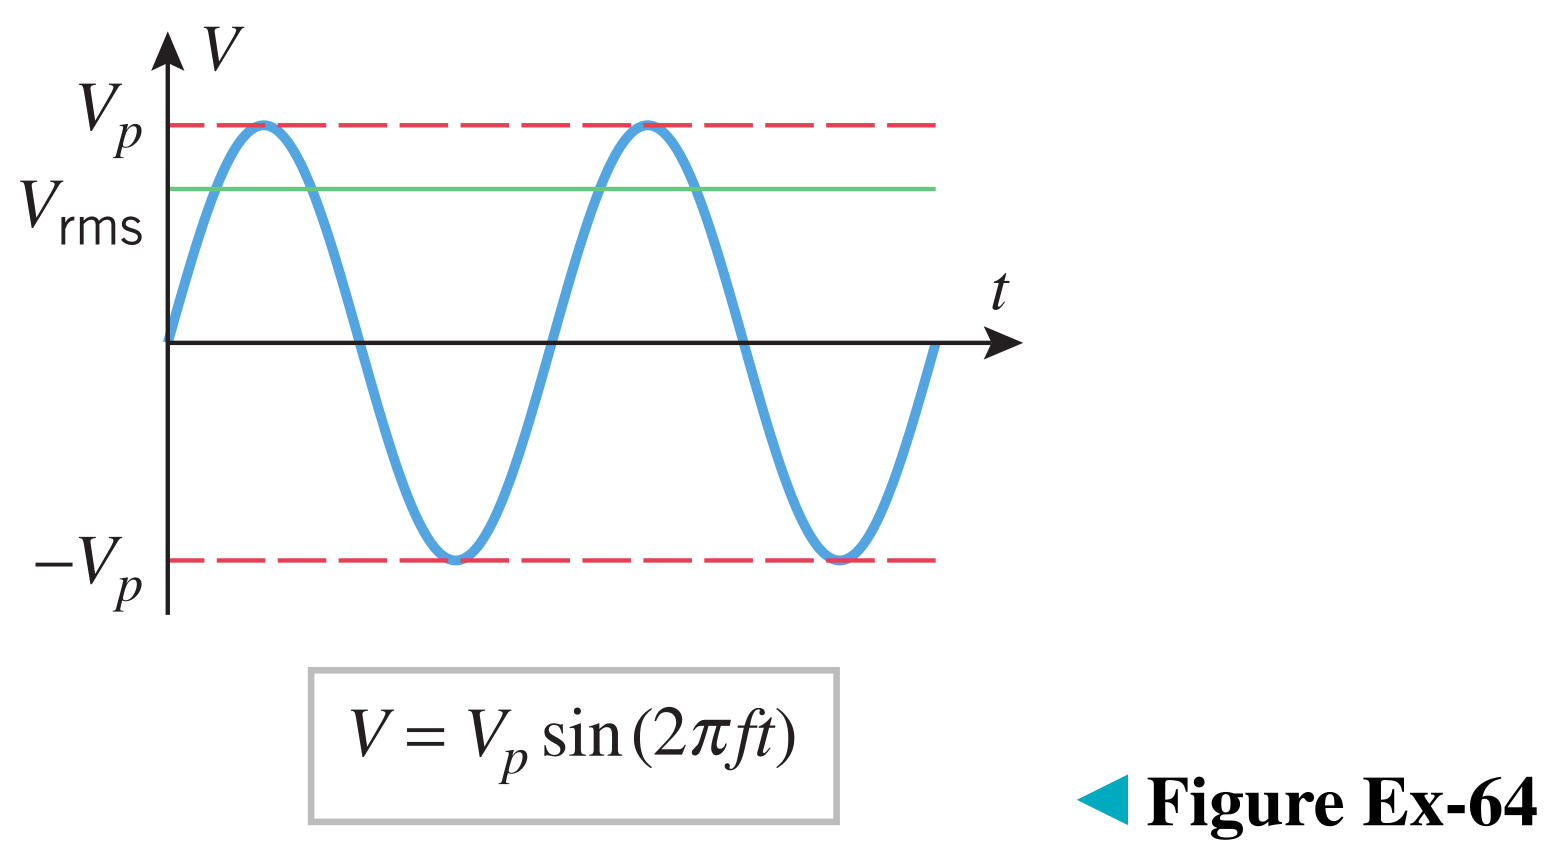
\includegraphics[width=0.7\textwidth]{../img/img_Lista4/1_64.png}
\end{figure}

La electricidad se suministra a los hogares en forma de \textbf{\textit{corriente alterna}}, lo que significa que el voltaje tiene una forma de onda sinusoidal descrita por una ecuación de la forma
\[
V = V_p \sin{(2\pi ft)}
\]
(ver la figura adjunta). En esta ecuación, $V_p$ se llama \textbf{\textit{voltaje máximo}} o \textbf{\textit{amplitud}} de la corriente, $f$ se llama \textbf{\textitfrecuencia}} y $1/f$ se llama \textbf{\textit{período}}. Los voltajes $V$ y $V_p$ se miden en voltios ($V$), el tiempo $t$ se mide en segundos ($s$) y la frecuencia se mide en hercios ($Hz$). ($1 Hz = 1$ ciclo por segundo; un \textbf{\textit{ciclo}} es el término eléctrico para un período de la forma de onda). La mayoría de los voltímetros de corriente alterna leen lo que se llama \textbf{\textit{rms}} o \textbf{\textit{valor cuadrático medio}} de $V$. Por definición, ésta es la raíz cuadrada del valor promedio de $V^2$ durante un período.
\begin{enumerate}[label=(\alph*)]
\item Demuestre que
  \[
  V_{rms}=\frac{V_p}{\sqrt{2}}
  \]
    [\textit{Sugerencia}: Calcule el promedio durante el ciclo de $t= 0$ a $t = 1/f$ y use la identidad $\sin^2{\theta}= \frac{1}{2}(1-\cos{2\theta})$ para ayudar a evaluar la integral.]
  
\item En Estados Unidos, los enchufes eléctricos suministran corriente alterna con un voltaje $rms$ de $120 V$ a una frecuencia de $60 Hz$. ¿Cuál es el voltaje máximo en tal toma corriente?


%Segunda parte de la lista de problemas
\subsection*{\centering \textbf{ \LARGE Segunda Parte} }
%% Sección 5.10: ejercicios 25, 26 y 27.
%% Sección 7.2: ejercicios 53, 54, 60 y 62.
  %% Sección 7.7: ejercicios 31, 32 y 34.
%% 5.10 -----------------------------------------------------------------------------------------------------------------------------------------------------------------------------------------------------------------------------
\section{Sección 5.10 \\Logaritmos y otras funciones definidas por integrales} 
% 25  -------------------------------------------------------------------------------------------------------------
\subsection{Ejercicio 25} Flores Morán Julieta Melina   \\
Usa los resultados del ejercicio 24 para encontrar la derivada:\\
\[
\frac{d}{dx} \int_x^{\pi} cos(t^{3}}) dt
\]
Cabe poner a consideración que el ejercicio 24 pide demostrar las siguiente propiedades:
\[
\frac{d}{dx} \left[ \int_x^{a} f(t) dt \right] = -f(x)
\]
 \[
\frac{d}{dx} \left[ \int_{g(x)}^{a} f(t) dt \right] = -f(g(x))g'(x)
\]
De las cuales usaremos la primera, donde  $f(t) = cos(t^3) \rightarrow f(x) = cos(x^3)$.De aquí que:
\[
\frac{d}{dx} \int_x^{\pi} cos(t^{3}}) dt = -cos(x^3)
  \]
  %% 26 --------------------------------------------------------------------------------------------------------------
  %% 27 ---------------------------------------------------------------------------------------------------------------
\subsection{Ejercicio 27} Flores Morán Julieta Melina \\
Encuentra
\[
\frac{d}{dx} \left[ \int_{3x}^{x^2} \frac{t-1}{t^2+1} dt \right]
\]
escribiendo
\[
\int_{3x}^{x^2} \frac{t-1}{t^2+1} dt = \int_{3x}^{0} \frac{t-1}{t^2+1} + \int_{0}^{x^2} \frac{t-1}{t^2+1} dt
\]
Entonces, podemos reescribir el problema de la siguiente manera:
\[
\frac{d}{dx} \left[ \int_{3x}^{x^2} \frac{t-1}{t^2+1} dt \right] = \frac{d}{dx} \left[\int_{3x}^{0} \frac{t-1}{t^2+1} dt\right]  + \frac{d}{dx} \left[ \int_{0}^{x^2} \frac{t-1}{t^2+1} dt \right]
\]
Podemos usar la propiedad
 \[
\frac{d}{dx} \left[ \int_{g(x)}^{a} f(t) dt \right] = -f(g(x))g'(x)
\]
Y para $\frac{d}{dx} \left[\int_{3x}^{0} \frac{t-1}{t^2+1} dt\right]$ podemos considerar $g(x) = 3x$, $f(t) = \frac{t-1}{t^2+1}$.

\begin{align*}
  \frac{d}{dx} \left[\int_{3x}^{0} \frac{t-1}{t^2+1} dt\right]
  & = - f(g(x))g'(x) \\
  & = - f(3x) \frac{d}{dx} 3x \\
  & = -  \frac{3x-1}{(3x)^2+1} \cdot 3 \\
  & = -  3 \cdot \frac{3x-1}{9x^2+1}
\end{end*}


Para $\frac{d}{dx} \left[ \int_{0}^{x^2} \frac{t-1}{t^2+1} dt \right]$, necesitamos que cumpla con las características para aplicar la propiedad de arriba. Esto lo logramos intercambiando los límites y cambiando el signo, así.
\[
 \int_{0}^{x^2} \frac{t-1}{t^2+1} dt = -  \int_{x^2}^{0} \frac{t-1}{t^2+1} dt
\]
Y
\[
\frac{d}{dx} \left[ \int_{0}^{x^2} \frac{t-1}{t^2+1} dt \right] = -\frac{d}{dx} \left[ \int_{x^2}^{0} \frac{t-1}{t^2+1} dt  \right]
\]
podemos considerar $g(x) = x^2$, $f(t) = \frac{t-1}{t^2+1}$.

\begin{align*}
  -\frac{d}{dx} \left[ \int_{x^2}^{0} \frac{t-1}{t^2+1} dt  \right]
  & = - (- f(g(x))g'(x)) \\
  & = f(x^2) \frac{d}{dx} x^2 \\
  & =   \frac{x^2-1}{(x^2)^2+1} \cdot 2x \\
  & = 2x \cdot \frac{x^2-1}{x^4+1}
\end{align*}

Así con estos resultados obtenemos que:
\begin{align*}
  \frac{d}{dx} \left[ \int_{3x}^{x^2} \frac{t-1}{t^2+1} dt \right]
  & =\frac{d}{dx} \left[\int_{3x}^{0} \frac{t-1}{t^2+1} dt\right]  + \frac{d}{dx} \left[ \int_{0}^{x^2} \frac{t-1}{t^2+1} dt \right] \\
  & = -  3 \cdot \frac{3x-1}{9x^2+1} + 2x \cdot \frac{x^2-1}{x^4+1}
\end{align*}
%% 7.2 -----------------------------------------------------------------------------------------------------------------------------------------------------------------------------------------------------------------------------
\section{Sección 7.2 \\Integración por partes} 
% 54  -------------------------------------------------------------------------------------------------------------
\subsection{Ejercicio 54} Flores Morán Julieta Melina  \\
Evaluá por partes la integral
\[
\int_0^{1} \frac{x^3}{\sqrt{x^2+1}}dx
\]
Usando:
\begin{enumerate}
\item Integración por partes\\
  Para usar la fórmula de integración por partes para esta integral definida
  \[
  \int_a^b u dv = uv \Bigg|_a^b - \int_a^b vdu
  \]
  Hay que elegir una u y una v. En este caso si $v=\sqrt{x^2+1} \rightarrow dv = \frac{x}{\sqrt{x^2+1}}dx$ y $u=x^2 \rightarrow du = 2xdx$ completa la integral que buscábamos. Usando la fórmula.
   \[
   \int_0^1 x^2  \frac{x}{\sqrt{x^2+1}} dx = x^2 \cdot \sqrt{x^2+1}  \Bigg|_0^1 - \int_0^1 \sqrt{x^2+1} \cdot 2xdx  \]

   La integral $\int_0^1 \sqrt{x^2+1} 2xdx $ es fácil obtenerla por sustitución. Si $u = x^2+1 \rightarrow du = 2x dx$. Así
   \begin{align*}
     \int_0^1 2x\sqrt{x^2+1} dx
     & = \int_{u(0)}^{u(1)} \sqrt{u} du\\
     & = \int_{1}^{2} u^{1/2} du\\
     & = \frac{2u^{3/2}}{3} \Bigg|_1^2\\
     & = \frac{2\cdot 2^{3/2}}{3} - \frac{2\cdot1^{3/2}}{3} \\
     & = \frac{4 \cdot \sqrt{2}}{3} - \frac{2}{3} \\
     & = \frac{4}{3}  \sqrt{2} - \frac{2}{3} \\
   \end{align}
   Entonces tenemos
   \begin{align*}
     x^2 \cdot \sqrt{x^2+1}  \Bigg|_0^1 - \int_0^1 \sqrt{x^2+1} \cdot 2xdx
     & =1^2 \cdot \sqrt{1^2+1} -[0^2 \cdot \sqrt{0^2+1} ] - [\frac{4}{3}  \sqrt{2} - \frac{2}{3}] \\
     & = 1 \cdot \sqrt{2}  - \frac{4}{3}  \sqrt{2} + \frac{2}{3} \\
     & =  -  \frac{1}{3} \sqrt{2}    + \frac{2}{3}
   \end{align*}
  
 \item Sustitución de $u= \sqrt{x^2+1}$ \\
   En este caso cabe tener en cuenta que $du = \frac{x}{\sqrt{x^2+1}}dx $
     \begin{align*}
       \int_0^{1} \frac{x^3}{\sqrt{x^2+1}}dx
       & = \int_{u(0)}^{u(1)} (u^2-1)du \\
       & = \int_{1}^{\sqrt{2}} (u^2-1)du \\
       & = \int_{1}^{\sqrt{2}} u^2 du - \int_{1}^{\sqrt{2}}  du \\
       & = \left (\frac{u^3}{3}  -  u \right) \Bigg|_1^{\sqrt{2}}\\
       & = \frac{\sqrt{2}^3}{3}  -  \sqrt{2} - \left[\frac{1^3}{3}  -  1 \right]\\
       & = \frac{2}{3}\sqrt{2}  -  \sqrt{2} - \frac{1}{3}  +  1\\
       & = -\frac{1}{3}\sqrt{2} + \frac{2}{3}  \\
   \end{align*}
\end{enumerate}
% 62  -------------------------------------------------------------------------------------------------------------
\subsection{Ejercicio 62} Flores Morán Julieta Melina  \\
Usa la formula (9)
\[
\int \cos^n dx = \frac{1}{n}\cos^{n-1}x \sin x+\frac{n-1}{n} \int cos^{n-2}x dx
\]
de reducción para evaluar
\begin{enumerate}
\item
\[
  \int cos^5x dx
  \]

  Para esto necesitamos el valor de $\int cos^{3}x dx$.
  \begin{align*}
   \int  cos^3x dx
   & = \frac{1}{3}\cos^{2}x \sin x+\frac{2}{3} \int cos^{1}x dx \\
   & = \frac{1}{3}\cos^{2}x \sin x+\frac{2}{3} senx + C
  \end{align*}
  Así que volviendo al problema original
   \begin{align*}
    \int cos^5x dx
    & = \frac{1}{5}\cos^{4}x \sin x+\frac{4}{5} \int cos^{3}x dx\\
    & = \frac{1}{5}\cos^{4}x \sin x+\frac{4}{5} \left[\frac{1}{3}\cos^{2}x \sin x+\frac{2}{3} \sen x \right]\\
     & = \frac{1}{5}\cos^{4}x \sin x+ \frac{4}{15}\cos^{2}x \sin x+\frac{8}{15} \sen x + C
  \end{align*}
\item
 \[
  \int_0^{\frac{\pi}{2}} cos^6x dx
  \]
  Evaluaremos primero $ \int cos^6x dx$, para lo cual necesitamos conocer
  \begin{align*}
   \int  cos^2x dx
   & = \frac{1}{2}\cos^{1}x \sin x+\frac{1}{2} \int cos^{0}x dx \\
   & = \frac{1}{2}\cos^{1}x \sin x+\frac{1}{2} \int dx \\
   & = \frac{1}{2}\cos x \sin x+\frac{1}{2} x + C \\
  \end{align*}
  
  \begin{align*}
   \int  cos^4x dx
   & = \frac{1}{4}\cos^{3}x \sin x+\frac{3}{4} \int cos^{2}x dx \\
   & = \frac{1}{4}\cos^{3}x \sin x+\frac{3}{4} \left[ \frac{1}{2}\cos x \sin x+\frac{1}{2} x \right]\\
    & = \frac{1}{4}\cos^{3}x \sin x+ \frac{3}8\cos x \sin x+\frac{3}{8} x + C\\
  \end{align*}
  Y ya podemos resolver fácilmente para n=6.
  \begin{align*}
   \int  cos^6x dx
   & = \frac{1}{6}\cos^{5}x \sin x+\frac{5}{6} \int cos^{4}x dx \\
   & = \frac{1}{6}\cos^{5}x \sin x+\frac{5}{6} \left[ \frac{1}{4}\cos^{3}x \sin x+ \frac{3}8\cos x \sin x+\frac{3}{8} x  \right]\\
   & = \frac{1}{6}\cos^{5}x \sin x+ \frac{5}{24}\cos^{3}x \sin x+ \frac{15}{48}\cos x \sin x+\frac{15}{48} x \\
   & = \frac{1}{6}\cos^{5}x \sin x+ \frac{5}{24}\cos^{3}x \sin x+ \frac{5}{16}\cos x \sin x+\frac{5}{16} x + C \\
   \end{align*}
    Ahora hay que evaluarlo en los límites dados
    \begin{align*}
   \int_0^{\frac{\pi}{2}}cos^6x dx
   & = \left [\frac{1}{6}\cos^{5}x \sin x+ \frac{5}{24}\cos^{3}x \sin x+ \frac{5}{16}\cos x \sin x+\frac{5}{16} x \right] \Bigg|_0^{\frac{\pi}{2}}\\
   & =  \frac{1}{6}\cos^{5}  \left( \frac{\pi}{2} \right) \sin \left( \frac{\pi}{2} \right)+ \frac{5}{24}\cos^{3}\left( \frac{\pi}{2} \right) \sin \left( \frac{\pi}{2} \right)  \\
     & + \frac{5}{16}\cos \left( \frac{\pi}{2} \right) \sin \left( \frac{\pi}{2} \right)+\frac{5}{16} \left( \frac{\pi}{2} \right)\\
   &  - \left [\frac{1}{6}\cos^{5} 0 \sin 0+ \frac{5}{24}\cos^{3}0 \sin 0+ \frac{5}{16}\cos 0 \sin 0+\frac{5}{16} 0 \right] \\
   & = \frac{5}{16} \left( \frac{\pi}{2} \right) \\
   & = \fra\frac{5}{16}c{5 \pi}{32}
   \end{align*}
\end{enumerate}
%% 7.7 -----------------------------------------------------------------------------------------------------------------------------------------------------------------------------------------------------------------------------
\section{Sección 7.7 \\Integración numérica: Regla de Simpson} 
% 32  -------------------------------------------------------------------------------------------------------------
\subsection{Ejercicio 32} Flores Morán Julieta Melina  \\
El valor exacto de la integral dada es $\pi$ (verificar). Aproximar la integral usando (a) la aproximación del punto medio$ M_{10}$, (b) la aproximación trapezoidal $T_{10}$, y (c) Aproximación de la regla de Simpson $ S_{20}$ usando la Fórmula (7). Aproximar el error absoluto y expresa tus respuestas con al menos cuatro decimales.
\[
\int_0^3 \frac{4}{9} \sqrt{9-x^2} dx
\]
\begin{enumerate}
\item Verificar el valor de la integral dada, esta es una integral del formulario, entonces usamos la formula.
   \begin{align*}
     \int_0^3 \frac{4}{9} \sqrt{9-x^2} dx
     & = \frac{4}{9}  \int_0^3 \sqrt{9-x^2} dx \\
     & = \frac{4}{9}  \left[ \frac{x}{2} \sqrt{9-x^2} + \frac{9}{2} \sin ^{-1} {\frac{x}{3}} \right] \Bigg|_0^3  \\
     & = \left[ \frac{4x}{18} \sqrt{9-x^2} + \frac{36}{18} \sin^{-1} {\frac{x}{3}}\right]  \Bigg|_0^3   \\
     & = \left[ \frac{2x}{9} \sqrt{9-x^2} + 2 \sin^{-1} {\frac{x}{3}} \right] \Bigg|_0^3  \\
     & = \left[ \frac{2 \cdot 3}{9} \sqrt{9-3^2} + 2 \sin^{-1} {\frac{3}{3}} \right] - \left[ \frac{2 \cdot 0}{9} \sqrt{9-0^2} + 2 \sin^{-1} {\frac{0}{3}} \right] \\
     & = \left[ \frac{2}{3} \sqrt{9-9} + 2 \sin^{-1} {1} \right] - \left[  2 \sin^{-1} {0} \right] \\
     & = \left[ 2 \cdot \frac{\pi}{2} \right] - \left[  2 \cdot 0 \right] \\
     & = \pi
   \end{align*}
 \item Aproximar la integral
   \begin{enumerate}
   \item $M_{10}$ \\
     Este método se describe de la siguiente forma:
     \[
     M_n = \left( \frac{b-a}{n} \right) \sum_{k=1}^{n}f(x_k^*)
     \]
     \[
     x_k^* = \frac{1}{2}(x_{k-1} + x_k)
     \]
     \begin{figure}[H]
       \centering
       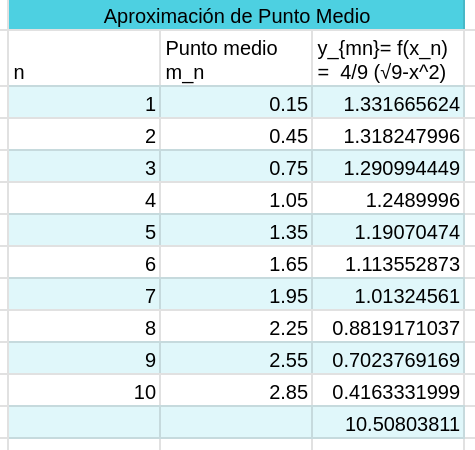
\includegraphics[width=0.7\textwidth]{../img/img_Lista4/MP.png}
     \end{figure}
     \[
      M_{10} =  (0.30)(10.0803811)= 3.152411433
     \]
   \item $T_{10}$ \\
     Usaremos la definición que dice que
     \[
     T_n = \left( \frac{b-a}{2n}\right)[y_0 + 2y_1 + \ldots +2 y_{n-1} + y_n]
     \]
     \begin{figure}[H]
       \centering
       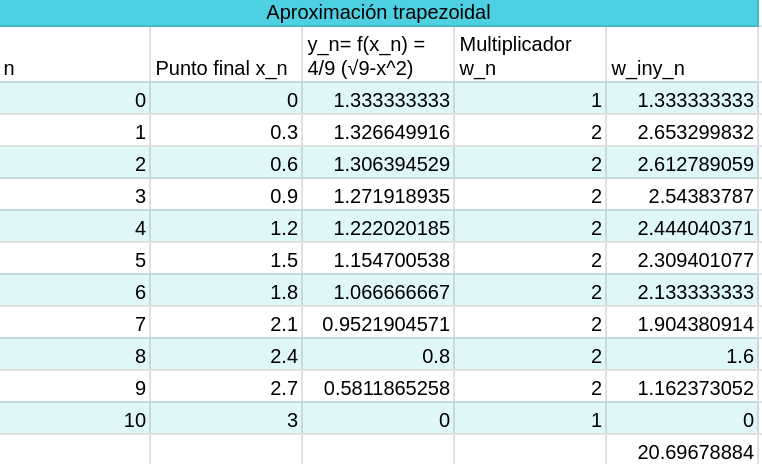
\includegraphics[width=0.7\textwidth]{../img/img_Lista4/TN1.png}
     \end{figure}
      \[
      T_{10} =  (0.15)(20.69678884)= 3.104518326
      \]
      
   \item $S_{20}$ \\
     Este método se basa en los anteriores y se describe como sigue
     \[
     S_n = S_{2k} = \frac{1}{3} (2M_k + T_k)
     \]
     En este caso tenemos que con lo ya calculado:
     \[
     S_{20} = S_{2 ~10} = \frac{1}{3} (2M_{10} + T_{10})
     \]
      \[
     S_{20} = 3.136447064
     \]
    \end{enumerate}
 \item Error absoluto
    \begin{enumerate}
   \item $|M_{10}| = |\pi - M_{10}| \approx |-0.010807| = 0.010807$
   \item $|T_{10}|  = |\pi - T_{10}| \approx |0.0370926| = 0.0370926 $
    \item $|S_{20}|  = |\pi - S_{20}| \approx |0.0051455| = 0.0051455 $
   \end{enumerate}
\end{enumerate}
\end{document}

